\documentclass[11pt]{article}
\usepackage{geometry}                % See geometry.pdf to learn the layout
\usepackage{graphicx}
\usepackage{amssymb}
\usepackage{epstopdf}

\title{Compte-rendu du TEA n°4}
\author{\textsc{Valentin GAUTHIER}\\ Alexandre TORRES--LEGUET}

\begin{document}
\maketitle

\section{Introduction}
%présentation du problème, le contexte

\quad \quad Ce compte-rendu présente le travail réalisé dans le cadre du TEA 4 de l'enseignement d'AAP, qui se concentre sur les tas en \textsc{C}, notamment le tri par tas et le codage de Huffman.

\section{Développement}
%organisation du programme
%organisation du groupe (qui a fait quoi)
%difficultés

\subsection{Programme 1 : tri par tas}

\quad \quad Le dossier \texttt{codage} recense notre travail relatif au tri par tas.\\

Nous avons vu en TD le fonctionnement et l'implémentation du tri par tas à l'aide du type \texttt{T\textunderscore heap}. Nous avons fait le choix de l'implémenter d'une autre manière, plus courte, qui ne dépend pas d'un type spécialisé pour un tas. Notre implémentation se base sur la fonction \texttt{tassifier}.

Cette fonction modifie le tableau (qui représente le tas) en place afin de maintenir la propriété de maximier/minimier. Elle suppose que seule l'élément \texttt{root}, noeud sur lequel on l'appelle, n'est pas à la bonne place dans le tas. Elle s'appelle donc récursivement pour "faire descendre" \texttt{root} dans le tas à sa bonne place.

Ensuite, nous avons développé la fonction \texttt{heap\textunderscore sort} qui effectue le tri d'un \texttt{T\textunderscore data}.
Cette fonction commence par modifier le tableau à trier afin de lui donner la propriété de maximier/minimier. Pour cela, elle remonte le tas en appellant \texttt{tassifier} à chaque rencontre de noeud. Ensuite, le tri s'effectue en \texttt{n} étapes : à chaque début d'étape, on sait que la propriété de maximier/minimier est vraie, donc la racine du tas est l'élément le plus grand/petit : on le met de côté (on l'échange avec le dernier élément), on sait qu'il est alors à sa place finale. On appelle alors \texttt{tassifier} pour retrouver la propriété maximier/minimier. On passe alors à l'étape suivante.

\subsection{Programme 2 : codage}

\quad \quad Le dossier \texttt{codage} recense notre travail relatif à la première partie du codage de Huffman. \\

Le programme demandé doit lire une chaîne de caractère sur l'entrée standard, et afficher sur la sortie standard le code de chaque caractère, le text codé, ainsi qu'une conclusion sur le ratio de compression.

Nous avons pour cela dû manipuler un tas indirect : les noeuds du tas sont les caractères, mais la valeur que l'on regarde pour savoir si un noeud est plus grand qu'un autre ne doit pas être le code \texttt{ASCII} du noeud, mais plutôt l'occurence du caractère du noeud dans la chaîne de caractères à coder : c'est en cela que l'on parle de tas \textbf{indirect}.

La seule modification majeure pour passer du tas normal implémenté en cours au tas indirect se situe dans les fonctions \texttt{siftDown} et \texttt{siftUp} et dans les fonctions macros utilisées. En effet, le tas du TD utilisait les fonction macros \texttt{VAL} et \texttt{VALP} qui retournaient la valeur du noeud à partir de la composante \texttt{tree} du tas. Nous avons donc simplement utilisé deux nouvelles macros \texttt{VAL\textunderscore ih} et \texttt{VALP\textunderscore ih} (\texttt{ih} pour \textbf{i}ndirect \textbf{h}eap) qui retourne la valeur du noeud à partir de la composante \texttt{data} du tas indirect (qui recense les occurences des caractères).

Une fois cette constatation faite, nous avons alors suivi l'exemple détaillé de la séance 4 (\texttt{ABBACADABRA}) pour en déduire l'algorithme à suivre afin de générer l'arbre de Huffman.

Une fois cela fait, nous nous sommes attardés sur la partie visualisation du programme. Il s'agit essentiellement de beaucoup de formatages, avec des manipulations de chaînes de caractères. Nous avons utilisé la fonction \texttt{int system(const char *command)} (décrite dans la consigne du TEA 3) pour générer les fichiers \textsc{PNG} une fois les fichiers \textsc{DOT} écrits. Nous nous sommes inspirés de la fonction \texttt{showHeap\textunderscore rec} vue en TD qui travaille récursivement pour afficher un tas.

\subsection{Programme 3 : Huffman}

\quad \quad Le dossier \texttt{huffman} recense notre travail relatif au problème 3 sur le codage de Huffman. \\

Nous avons dans cette partie réutilisé beaucoup des fonctions développées lors du problème 2, notamment pour la construction de l'arbre de codage. \\

Pour la partie compressage du programme (lorsqu'on donne une fichier source et un fichier target au programme), il s'agit dans un premier temps de construire l'arbre de codage, déduire les codes de chacun des caractères, puis créer l'entête à partir de l'arbre de codage, c'est-à-dire la suite de 0 et de 1 (\texttt{parcours\textunderscore prefixe} dans le code), et la suite des caractères (\texttt{caracteres} dans le code). C'est ce dont se charge la fonction \texttt{huffmanTree\textunderscore to\textunderscore entete}, qui travaille récursivement.\\

Pour la partie décompressage du programme, il s'agit dans un premier temps de lire et de stocker séparément le parcours préfixe et les caractères stockés dans l'entête de Huffman du fichier à décompresser. Une fois cela fait, on utilise la fonction \texttt{entete\textunderscore to\textunderscore huffmanTree}, qui construit l'arbre de codage à partir d'une entête. Cette fonction travaille également récursivement et utilise des pointeurs pour savoir notamment, dans tous les appels récursifs, quelle position de la chaîne de caractère de \texttt{parcours\textunderscore prefixe} elle doit lire. Une fois cela fait, on dispose de l'arbre de codage et on peut alors calculer les codes de chacun des caractères. Alors, on peut déchiffrer facilement le texte codé en le parcourant et en détectant le plus petit code connu (ce qui est possible car aucun code de Huffman n'est préfixe d'un autre). \\

Ces deux algorithmes (implémentés dans les fonctions \texttt{huffmanTree\textunderscore to\textunderscore entete} et \\ \texttt{entete\textunderscore to\textunderscore huffmanTree}) sont le fruit de quelques dizaines de minutes passés avec un papier et un crayon sur des exemples simples pour en déduire une méthode générale. \\

Nous nous sommes aidés en ligne pour savoir comment accéder et lire un fichier. Nous avons appris l'existence de fonctions telles que \texttt{fopen}, \texttt{fseek} et \texttt{fclose}. \\

Alors que nous pensions avoir terminé cette partie, nous avons eu la mauvaise surprise de constater que notre algorithme ne fonctionnait pas lorsque le texte à compresser comportait un ou plusieurs caractères retour chariot \textbf{\textbackslash n}. En effet, la partie compressage fonctionne bien : l'entête comporte bien le parcours préfixe de l'arbre de codage, et la liste des caractères présents. Cependant, cette liste comporte alors un retour chariot : elle s'étale donc sur deux lignes dans l'entête de Huffman. Nous n'avions pas pris en compte ce cas dans le décompressage d'un fichier : pour nous, la liste des caractères ne pouvait s'étaler que sur une seule ligne.
Il a donc fallu trouver une solution à ce problème. Nous en avons envisagé deux :
\begin{itemize}
\item remplacer, dans l'entête d'Huffman, \textbf{\textbackslash n} par un autre caractère (de préférence très peu utilisé). Ainsi la liste des caractères tiendrait sur une seule ligne. Cela nous aurait obligé à traiter séparément ce caractère.
\item compter le nombre de lignes dans le fichier à décompresser. Dans le cas normal (pas de \textbf{\textbackslash n} dans le texte original qui a été compressé), le fichier à décompresser comporte 3 lignes : une ligne sur laquelle sur trouve le parcours préfixe de l'arbre de codage, une ligne sur laquelle se trouve les caractères du texte et une ligne sur laquelle se trouve le texte codé. Si on compte 4 lignes dans le fichier à décompresser, on sait alors que le texte original comportait au moins un \textbf{\textbackslash n}. On peut alors s'adapter et, lors de la lecture de la liste des caractères dans l'entête, lire 2 lignes plutôt qu'une. C'est la solution que nous avons choisi.
\end{itemize}


\subsection{Organisation - Gestion de projet}

Concernant l'organisation des tâches au sein du groupe, nous avons travaillé ensemble, lors la semaine suivant la séance 4 du TD, sur la partie tri par tas.

Puis, pendant les vacances, nous avons revus individuellement en détail le poly de la séance 4 sur le codage de Huffman avant de nous lancer sur les problèmes 2 et 3. Nous avons contribué de façon équivalente à ces deux problèmes, en répartissant les tâches en "sous-problèmes" (\textbf{ex :} fonction qui construit l'arbre de codage, fonction qui calcule les codes, fonction qui génère les fichiers de visualisation etc...)

\section{Résultats}
%présentation des résultats, jeux d'essais, analyse, temps d'exec...
Voici le comportement de notre algorithme de tri par tas sur des tableaux de grande taille.
On observe bien un comportement quasi-linéaire, pour les tris de tableaux de nombres aléatoires aussi bien qu'ordonnés. 

\begin{center}
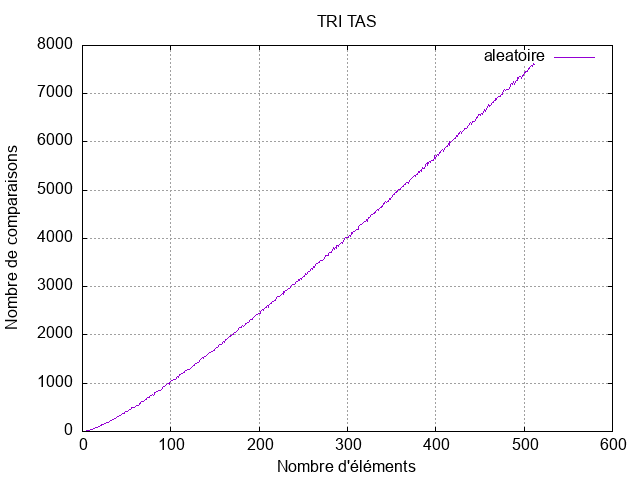
\includegraphics[scale=0.6]{images/Tri_tas_aleatoire_cmp.png}
\end{center}

\begin{center}
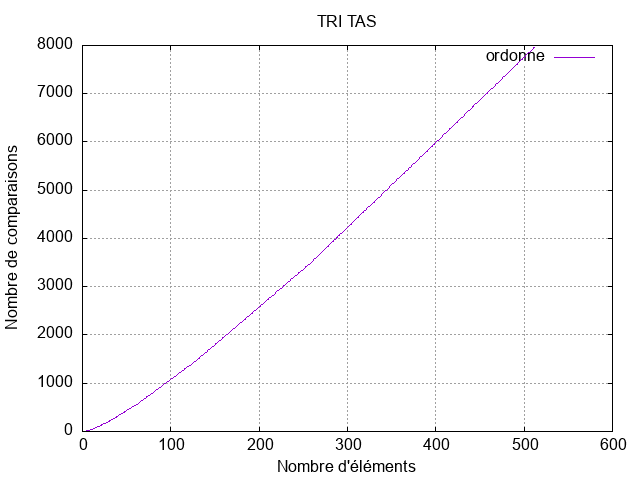
\includegraphics[scale=0.6]{images/Tri_tas_ordonne_cmp.png}
\end{center}

Nous avons enfin comparé expérimentalement les vitesses de tous les tris que nous avons implémentés jusqu'à alors : tri par tas, tri fusion et tri rapide, ainsi que le tri rapide disponible nativement en \textsc{C} via la fonction \texttt{qsort}. Pour cela, nous avons utilisé la bibliothèque \texttt{time} afin de mesurer le temps d'exécution de nos programmes. Les temps que l'on voit apparaître dans le tableau correspondent au tri de 100 tableaux de taille \texttt{MAX\textunderscore ELT = 250 000}.

\begin{center}
\begin{tabular}{||c c c c||} 
 \hline
 \texttt{quicksort} & \texttt{fusionsort} & \texttt{qsort} & \texttt{heap\textunderscore sort}\\ [0.5ex] 
 \hline\hline
11.2s & 12.1s & 4.1s & 8.1s \\ 
\hline
\end{tabular}
\end{center}

On remarque que notre tri par tas bat nos implémentations du tri fusion et du tri rapide du TEA 3. Toutefois, le tri natif \texttt{qsort} reste invaincu. Après avoir vu son code source, nous avons remarqué qu'il est implémenté sans récursivité, et l'on sait que la récursivité peut présenter un désavantage en terme de performances. Cela explique donc peut-être ces constatations.

Pour ce qui est des problèmes 2 et 3, nos algorithmes fonctionnent pour n'importe quel texte qu'on leur donne à compresser. Nous avons bien vérifié que notre programme \texttt{huffman.exe} arrive à décoder un texte qu'il a lui même codé. Le temps d'exécution semblent convenables, à noter que la génération d'images pour \texttt{codage.exe} rend son exécution beaucoup plus lente.

\section{Conclusion}
%analyser les problèmes, perspectives

\quad \quad Nous avons pu, au cours de ce TEA, renforcer notre compréhension du tri par tas puisque nous avons suivi une autre approche que celle offerte en TD. Egalement, nous avons pu passer du temps sur la manipulation de tas dans le cadre du codage de Huffman. Nous avons apprécié ce TD car il y avait beaucoup de "petits algorithmes" à développer que nous avons pu extrapoler à partir d'exemples simples avec un papier et un crayon.

\end{document}  
